\externaldocument{GEP/deliverable1.tex}

\section{Integración de OmpSs-2 en C/C++ COMPSs}

Con tal de realizar una buena integración necesitamos conocer bien cómo funcionan y/o cómo están hechos los componentes a integrar. Con tal de adquirir los conocimientos necesarios, vamos a indagar en la estructura interna del \textit{binding} de \textit{C/C++} de \textit{COMPSs} y a entender cómo se desarrolla y compila una aplicación. También deberemos ver cómo funciona la \textit{API} del \textit{runtime} de \textit{OmpSs-2} \textit{Nanos6} y el proceso habitual de desarrollo y compilado de una aplicación que utiliza el modo librería.

\subsection{Estructura de los bindings}

El \textit{runtime} de \textit{COMPSs} fue desarrollado en \textit{Java}, por lo que si queremos soportar cualquier lenguaje (salvo el propio \textit{Java}), necesitamos de alguna manera establecer comunicación con ese lenguaje. Es decir, necesitaremos un mecanismo que nos permita ejecutar código de este lenguaje a soportar, por supuesto, en ambas direcciones. 
\par\bigskip
Actualmente, \textit{COMPSs} cuenta con los \textit{bindings} de \textit{C/C++} y \textit{Python} (usualmente conocido como \textit{PyCOMPSs}), que utilizan estos mecanismos descritos anteriormente. Para efectuar la ejecución entre \textit{Java} y \textit{C/C++} se utiliza la \textit{Java Native Interface}, dado que desde \textit{Python} se puede utilizar la \textit{Python-C API} para , con un componente intermedio entre \textit{Python} y \textit{Java} escrito en \textit{C/C++} (utilizando la \textit{JNI}) permitiríamos efectuar llamadas desde \textit{C/C++} y \textit{Python} al \textit{runtime} y al revés. 
\par\bigskip
La siguiente imagen muestra la estructura general de los \textit{bindings} actuales. Las cajas representan componentes de la arquitectura, el color de cada caja ha sido escogido para representar un lenguaje, por lo que dos cajas del mismo color que estén conectadas directamente con un flecha no requieren de mecanismos adicionales.

\begin{figure}[H]
    \centering 
    \caption{Estructura de los bindings de COMPSs.}
    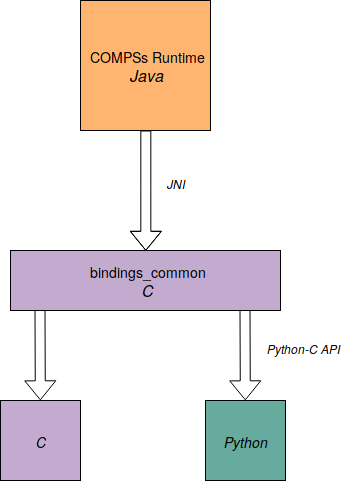
\includegraphics[scale=0.6]{estructuraBindings.png}
    \label{fig:estructurabindings}
\end{figure}

\subsection{Modelo de ejecución en el binding C/C++}
\label{sec:bindings}

\textit{C} y \textit{C++} son lenguajes de programación compilados, esto quiere decir que necesitamos un segundo programa llamado compilador que procese nuestro programa y genere un fichero que nuestro ordenador pueda ejecutar, a este proceso se le llama compilar y al fichero generado, binario. De esta manera, para poder obtener el modelo de ejecución introducido en la sección \ref{modeloejecucion}, necesitaremos compilar dos binarios, uno para el \textit{master} y otro para los \textit{workers}.
\par\bigskip

\begin{comment}
La aplicación que desarrolla el usuario, \textit{a priori} no envía las tareas a ejecutar ni las dependencias entre estas, no gestiona el \textit{runtime}, pero es desarrollada siguiendo unas directrices que nos permitirán generar código que sí gestione todo lo que es necesario con tal de que la aplicación se distribuya correctamente. 
\end{comment}

La aplicación que desarrolle el usuario, tiene que ser transparente al \textit{runtime}, para conseguirlo tan sólo se necesita una interfaz indicando las tareas a detectar al ejecutar la aplicación. Entonces, una vez compilemos la aplicación de COMPSs en C/C++, se generará automáticamente (a partir de ahora \textit{autogenerar}) código para las tareas, que gestionarán la comunicación con el \textit{runtime}.
\smallskip
La siguiente imagen describe de manera visual cómo se compila una aplicación. 

\begin{figure}[H]
    \centering 
    \caption{Proceso de compilación de una aplicación COMPSs C/C++.}
    %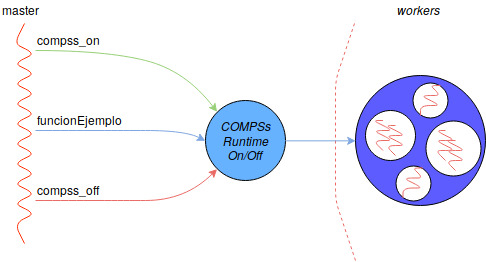
\includegraphics[width=\textwidth]{sta-masterworker.jpg}
    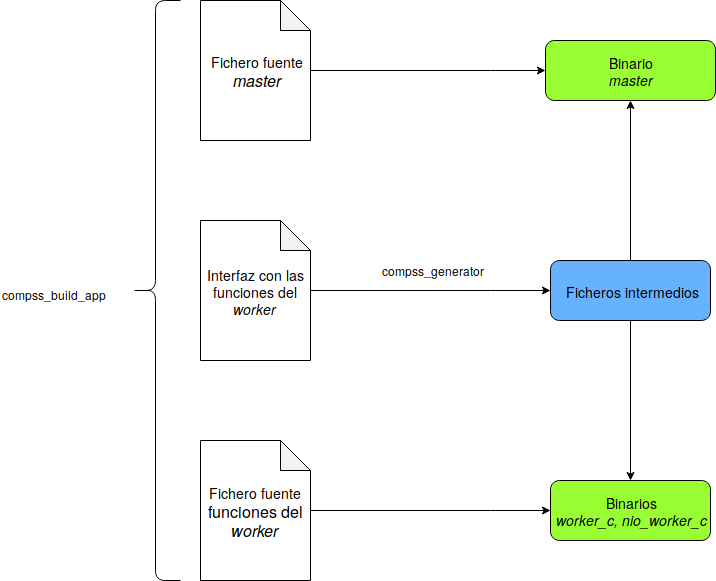
\includegraphics[scale=0.5]{workflowCompilado.png}
    \label{fig:workflowcompilado}
\end{figure}

\par\bigskip
Para facilitar el compilado de la aplicación se utiliza el script \textit{compss\_build\_app}, y para hacer la generación de código a partir de la interfaz, el binario \textit{compss\_generator}.
La aplicación una vez desarrollada por el usuario, compilada sin \textit{COMPSs} por el medio también funcionaría, pero sencillamente las tareas serían ejecutadas \textit{in situ} en el \textit{master}.  Lo que pretendemos hacer al introducir \textit{COMPSs} es que el \textit{master}, en vez de ejecutar la tarea, comunique al \textit{runtime} que se debe ejecutar una tarea, y este se encargue de ejecutarla en un \textit{worker}, todo evidentemente, de manera transparente al usuario.
\par\bigskip

\bigskip
En la figura \ref{fig:workflowcompilado} veíamos la caja negra de ficheros intermedios, estos ficheros son el \textit{stubs} y \textit{executor} (siempre del estilo, \textit{ejemplo-stubs.cc} y \textit{ejemplo-executor.cc} donde ejemplo es el nombre de la aplicación compilada). El fichero \textit{stubs} corresponde con la parte del \textit{master} que se encargará de comunicarse con el \textit{runtime} para registrar la tarea. Esto lo consigue implementando las funciones de las tareas con el código para gestionar su registro, es decir, sustituyendo el código que sería propio de la ejecución de cada tarea por un código para efectuar el registro en el \textit{runtime}. Una vez registrada la tarea, eventualmente el \textit{runtime} designará a un \textit{worker} a ejecutarla. El \textit{worker} recibirá la tarea que debe ejecutar, los datos necesarios y más parámetros, el \textit{executor} ha sido \textit{autogenerado} con el código principal de la aplicación, por lo que conoce como gestionar los datos y parámetros recibidos para ejecutar la tarea pertinente. 

\begin{comment}
\begin{figure}[H]
    \centering  
    \caption{Registro y ejecución de tareas en una aplicación COMPSs C/C++.}
    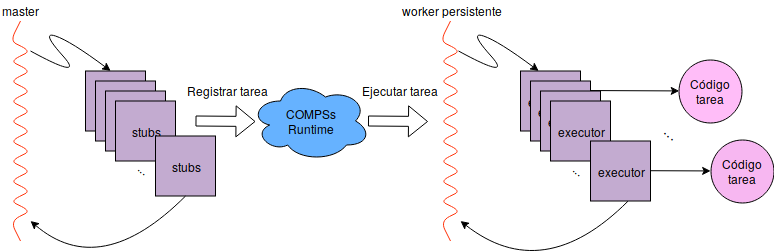
\includegraphics[scale=0.6]{stubs-executor.png}
    \label{fig:stubs-executor}
\end{figure}

La imagen anterior muestra las llamadas a funciones pertinentes a \textit{stubs} que contienen el código para registrar las tareas en el \textit{runtime}, la eventual ejecución de las tareas registradas en los \textit{workers} que haya disponibles y como toma parte su ejecución mediante el \textit{executor}. Ahora que sabemos como se estructura un \textit{binding}, y en concreto, como funciona el de \textit{C/C++}, el siguiente paso es estudiar el funcionamiento de \textit{OmpSs-2}.

%\subsection{Conceptos básicos de OmpSs-2}

\subsubsection{Mercurium}

\textit{Mercurium} es el encargado de compilar una aplicación de \textit{OmpSs-2} y hacer que las directivas insertadas en el código tengan efecto sobre este. De manera superficial, lo que hace es añadir código para gestionar el \textit{runtime}, encender el \textit{runtime}, añadir las tareas, notificar las dependencias y un largo etcétera. 

\subsubsection{Nanos6}

\todo{Pensar algo}
\end{comment}

\subsection{Modo librería: nanos6\_spawn\_function \label{spawnfunction}}

En la sección \ref{sec:bindings} dimos una visión más interna y propia de desarrollador del \textit{binding} de \textit{C/C++}. Sobre \textit{OmpSs-2} necesitamos saber, como se desarrolla una aplicación, en concreto con el modo librería.
\medskip

Esta funcionalidad, nos permite registrar una tarea en el \textit{runtime} de \textit{OmpSs-2} de manera asíncrona, con lo cuál podremos brindar a cada tarea y sus sucesoras un entorno aislado del resto. Gracias a esto, conseguiremos arreglar el problema con la migración de \textit{threads}, planteado en la sección \ref{compssompss}. \smallskip

\begin{lstlisting}[caption={Definición de la función nanos6\_spawn\_function.},captionpos=b, label={lst:nanos6spawn}, language=C++]
void nanos6_spawn_function(
   void (*function)(void *), 
   void *args,
   void (*completion_callback)(void *), 
   void *completion_args, 
   char const *label
);
\end{lstlisting}

La anterior imagen muestra la definición de la función que nos permitirá registrar una función \textbf{function} con argumentos \textbf{args} en el \textit{runtime}. Una vez ejecutada la función registrada como tarea, se ejecutará la función \textbf{completion\_callback} con argumentos \textbf{completion\_args} (mecanismo conocido como \textit{callback}, de ahí el nombre), el argumento de la función \textit{label} sirve para etiquetar la tarea con el nombre que contenga.

\subsubsection{Ejemplo}
\label{sec:ejemplo}

Con tal de entender como funciona un programa que utilice el modo librería, vamos a ver un ejemplo sencillo. Este programa de ejemplo, hará \textit{spawn} de una función y dentro de ésta se generarán tareas con dependencias entre ellas. \smallskip

\begin{lstlisting} [caption={Función a ser registrada como tarea.},captionpos=b, label={lst:nanos6ejemplo}, language=C++]
 int nanos6_ejemplo(int* a) {

    int local_a;

    #pragma oss task shared(local_a) out(local_a) 
    {
        local_a = a[0];
    }

    #pragma oss task shared(local_a) inout(local_a)
    {
        local_a = local_a * 4;
    }

    #pragma oss taskwait

    return local_a;
}
\end{lstlisting}

En la imagen podemos ver la función \textbf{nanos6\_ejemplo}, ésta tiene como parámetro un puntero a enteros \textbf{a} y retorna un valor del tipo \textbf{int}. La función será registrada como tarea desde otro fichero. El cálculo que se realiza en la función no tiene la menor importancia, es solo un \textbf{ejemplo}. \medskip

Por supuesto, esta función será compilada con \textit{Mercurium}, si no fuera el caso, la función se ejecutaría correctamente pero no se generarían las tareas de dentro de la función, por lo cuál la ejecución sería secuencial. 

\begin{lstlisting} [caption={Gestión del modo librería desde el main.},captionpos=b, label={lst:library-main}, language=C++]
    char const *error = nanos6_library_mode_init();
    if (error != NULL)
    {
        fprintf(stderr, "Error initializing Nanos6: %s\n", error);
        return 1;
    }

    condition_variable_t cond_var = COND_VAR_INIT;

    ejemplo_wrapper_args_t args;

    int A = 1;
    args.array = &A;
    
    nanos6_spawn_function(ejemplo_wrapper, &args, 
    					  condition_variable_callback, &cond_var, 
    					  "spawned ejemplo");

    wait_condition_variable(&cond_var);

    printf("%li\n", args.ret);

    nanos6_shutdown();

\end{lstlisting}

Las funciones \textit{nanos6\_library\_mode\_init()} y \textit{nanos6\_shutdown()} efectúan respectivamente el encendido y apagado del \textit{runtime}, el código que vemos entre estas dos llamadas es el correspondiente para registrar una función como tarea utilizando el modo librería. Dado que la función nanos6\_spawn\_function espera como un puntero los parámetros a pasar a la función, se deben incluir todos dentro de una estructura que los pueda contener, el \textit{struct} \textit{ejemplo\_wrapper\_args\_t} tiene los campos \textbf{a} y \textbf{ret} que corresponden al parámetro de la función \textit{nanos6\_ejemplo} y valor de retorno de ésta.

\bigskip
Un detalle que no se ha comentado es que la ejecución de este código será efectuada por \textit{pthreads}, el estándar \textit{POSIX} de \textit{threads}. Dado que la ejecución de la tarea tendrá lugar de manera \textbf{asíncrona} es necesario un mecanismo de sincronización, la implementación de \textit{threads} que utilizamos (y por tanto los mecanismos de sincronización dependerán de estos).

\bigskip

Requerimos de un mecanismo de sincronización por que la función que se registra como tarea la ejecuta un \textit{thread} diferente al que la registra, se hace uso de la librería \textit{pthread} \ref{appendix:pthread}.
\bigskip

\begin{comment}
\begin{figure}[H]
    \centering 
    \caption{Mecanismo de sincronización abstracto.}
    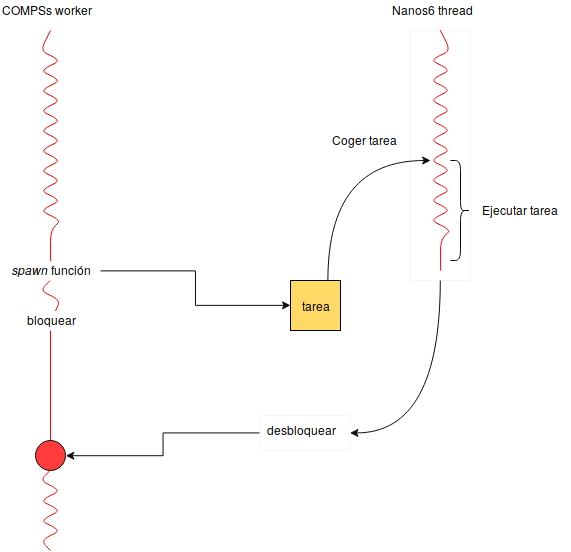
\includegraphics[scale=0.6]{spawn_sync.png}
    \label{fig:spawn\_sync}
\end{figure}
\end{comment}
 
\subsubsection{Mecanismo de sincronización} 
\label{sec:mecanismosync} 
Un \textit{thread} perteneciente al \textit{worker} de \textit{COMPSs} registra una tarea y un segundo thread perteneciente a \textit{OmpSs-2} espera a poder ejecutar alguna tarea. El primer \textit{thread} una vez haya registrado la tarea procederá a bloquearse, el segundo cuando acabe de ejecutar la tarea registrada, ejecutará un \textit{callback} donde desbloquearemos al primer \textit{thread}. \bigskip

El mecanismo abstracto es sencillo, pero la implementación real depende de los \textit{Pthreads}. Las estructuras utilizadas para realizar la sincronización son \textit{mutexes} y \textit{condition variables}. Un \textit{mutex} es una estructura que sirve para definir regiones de exclusión mútua mediante métodos de adquisición y liberación de la región, en este mecanismo se utilizan tan sólo por que son necesarios para utilizar \textit{condition variables}. Las \textit{condition variables} nos permiten que un \textit{thread} espere a un evento de manera no bloqueante, si no, habría que hacer \textit{polling} y consumir tiempo de cómputo inútilmente.
\bigskip

Será con las funciones \textit{pthread\_cond\_wait(pthread\_cond\_t * cond, pthread\_mutex\_t * mutex)} y \textit{pthread\_cond\_signal(pthread\_cond\_t * cond)} con las que respectivamente bloqueemos al primer \textit{thread} después de registrar la tarea y lo desbloqueemos al acabar de ejecutarla.
\bigskip

Dado que para utilizar \textit{condition variables} se necesitan \textit{mutexes} y se recomienda utilizar una variable auxiliar para evitar abrazos mortales (en el caso de que, el segundo \textit{thread} ya ha intentado desbloquear al primero, pero este aún no se había bloqueado, cuando se bloquee, se bloqueará para siempre), se crea una estructura de datos para contener todas estas variables llamada \textit{condition\_variable\_t}.

\smallskip

\begin{lstlisting} [caption={Definición de la estructura de datos condition\_variable\_t.},captionpos=b, label={lst:structwait-condition}, language=C++]
typedef struct {
    pthread_mutex_t _mutex;
    pthread_cond_t _cond;
    int _signaled;
} condition_variable_t;
\end{lstlisting}

\smallskip

\begin{lstlisting} [caption={Función wait\_condition\_variable},captionpos=b, label={lst:wait-condition}, language=C++]
void wait_condition_variable(condition_variable_t *cond_var)
{
    pthread_mutex_lock(&cond_var->_mutex);
    while (cond_var->_signaled == 0) {
        pthread_cond_wait(&cond_var->_cond, &cond_var->_mutex);
    }
    pthread_mutex_unlock(&cond_var->_mutex);
}
\end{lstlisting}

En la imagen \ref{lst:library-main} se utiliza la función \textit{wait\_condition\_variable(\&cond\_var)}, la llamada a  \textit{pthread\_cond\_wait} está dentro de una región crítica para prevenir que nadie más se bloquee sobre la misma \textit{condition variable} y esta se encuentra dentro de un \textit{while} por que puede ocurrir que el \textit{thread} se desbloquee sin haber sido desbloqueado por otro \textit{thread}, la variable \textit{cond\_var->\_signaled} será 0 hasta que el \textit{thread} que produzca el desbloqueo lo modifique, así garantizaremos que el desbloqueo es intencionado.
\smallskip

\begin{lstlisting} [caption={Callback de la tarea registrada},captionpos=b, label={lst:signal-condition}, language=C++]
void condition_variable_callback(void *untyped_arg)
{
    condition_variable_t *cond_var = (condition_variable_t *) 
    								 untyped_arg;

    pthread_mutex_lock(&cond_var->_mutex);
    cond_var->_signaled = 1;
    pthread_cond_signal(&cond_var->_cond);
    pthread_mutex_unlock(&cond_var->_mutex);
}
\end{lstlisting}

La imagen anterior muestra el \textit{callback} que se ejecuta al finalizar la ejecución de la tarea, modifica el valor de la variable \textit{cond\_var->\_signaled} y efectúa un \textit{pthread\_cond\_signal} para despertar al primer \textit{thread}.

\bigskip

Como es necesario utilizar una estructura auxiliar para pasar los parámetros mediante un puntero, necesitaremos también una función intermedia con la cuál llamar a la función que realmente queremos registrar como tarea. Habitualmente a este tipo de funciones intermedias se les llama \textit{wrapper}. En la siguiente imagen veremos la función que actúa como \textit{wrapper} de la función \textit{nanos6\_ejemplo}. \smallskip

\begin{lstlisting} [caption={Wrapper de la función nanos6\_ejemplo.},captionpos=b, label={lst:library-wrapper}, language=C++]
 void ejemplo_wrapper(void *untyped_arg)
{
    ejemplo_wrapper_args_t *args = 
        (ejemplo_wrapper_args_t *) untyped_arg;
    args->ret = nanos6_ejemplo(args->a);
}
\end{lstlisting}

El puntero de tipo \textit{void} puede contener cualquier tipo de estructura, aprovechando que sabemos que únicamente deberá contener el tipo \textit{ejemplo\_wrapper\_args\_t} se hace un \textit{cast} para interpretarlo como la estructura deseada. Se asigna \textbf{ret} al valor de retorno y se pasa \textbf{a} como parámetro.

\subsubsection{Compilado}
\label{sec:compilado}

El modo librería nos permite desacoplar de alguna manera la parte que pertenece a \textit{OmpSs-2} de la que no. Es decir, ahora podemos tener un código principal encargado de hacer \textit{spawn} de funciones que no tiene por qué estar compilado con \textit{Mercurium} y el \textit{flag} \textit{-{}-ompss-2}.
\par\bigskip

Un \textit{Makefile} para compilar el ejemplo \ref{sec:ejemplo} sería:
\medskip

\begin{lstlisting} [caption={Makefile para compilar el ejemplo.},captionpos=b, label={lst:makefileejemplo}, language=C++]                                                                                                                                               
all: ejemplo

# Codigo principal
main-ejemplo.o : main-ejemplo.c nanos6-ejemplo.h nanos6-helpers.h                                                                                                                                       
    $(CC) $(CFLAGS) -c main-ejemplo.c -o $@                                                                                                                                                                 

# Mecanismos de sincronizacion
nanos6-helpers.o : nanos6-helpers.c nanos6-helpers.h
    $(CC) $(CFLAGS) -c nanos6-helpers.c -o $@                                                                                                                                                                 

# Nanos6 (codigo a compilar con Mercurium y ompss-2)
nanos6-ejemplo.o :  nanos6-ejemplo.c nanos6-ejemplo.h
    $(MCC) $(CFLAGS) -c  nanos6-ejemplo.c -o $@                                                                                                                                                             

# Linking
ejemplo: main-ejemplo.o nanos6-ejemplo.o nanos6-ejemplo.o                                                                                                                                      
    $(CC) $^ -o $@ $(LIBS)                                                                                                                                                                                    
\end{lstlisting}

Se divide el \textit{Makefile} en cuatro etapas, la primera compila el \textit{main-ejemplo.c} utilizando el compilador definido por la variable de entorno \textit{CC}, en nuestro caso será \textit{g++}, la segunda etapa compila las funciones utilizadas para los mecanismos de sincronización descritos anteriormente en el fichero \textit{main-helpers.c}, la tercera compila el código que contiene la o las funciones a ser ejecutadas como tarea con el compilador definido por la variable de entorno \textit{MCC}, que es \textit{Mercurium}, y por último en una fase de \textit{linking} se enlazan los objetos compilados entre sí, y además con el objeto \textit{nanos6-library-mode.o} y la librería \textit{nanos6}, esto es necesario por que el objeto generado al compilar el \textit{main-ejemplo.c} utiliza las llamadas para encender el modo librería descritas en la sección \ref{sec:ejemplo}.

\subsection{Integración}

Ahora que tenemos claro el funcionamiento de ambas partes, podemos plantear un prototipo de la integración e implementarlo. Está claro que \textit{OmpSs-2} tomará parte únicamente en los nodos del tipo \textit{worker}, ya que es dónde realmente se ejecutarán las tareas detectadas por el \textit{master}. 
\par\medskip

En el ejemplo para utilizar el modo librería \ref{spawnfunction}, aprendimos como activar el \textit{runtime} de \textit{OmpSs-2} en este modo y como ejecutar las tareas, por lo que bastará con activarlo en los \textit{workers} (persistente y no persistente) y modificar la generación del código \textit{executor} (queremos hacerlo en el \textit{worker}) para generar la misma estructura del ejemplo en cada tarea de la interfaz de la aplicación.
\par\medskip
Entonces, con la activación de \textit{OmpSs-2} en los nodos \textit{worker} conseguiremos la siguiente estructura y modelo de ejecución.

\begin{figure}[H]
    \centering 
    \caption{Estructura y modelo de ejecución master-worker de la integración COMPSs+OmpSs-2}
    %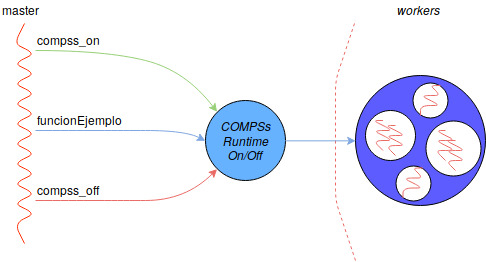
\includegraphics[width=\textwidth]{sta-masterworker.jpg}
    \includegraphics[scale=0.5]{compss2rt.png}
    \label{fig:compssompssrt}
\end{figure}

Durante la ejecución del programa principal se irá generando un grafo con las tareas que se deben ejecutar, eventualmente cada una de estas será enviada a un nodo \textit{worker} (en la figura tan sólo aparece uno, pero podrían ser más) y este ejecutará la tarea de \textit{COMPSs} en forma de tarea de \textit{OmpSs-2}.
La ejecución de las tareas de \textit{OmpSs-2} generará otro grafo, dónde figurarán tanto las tareas que han sido creadas mediante el mecanismo de \textit{spawn} como las que puedan ser creadas dentro de las anteriores, y finalmente las tareas de este grafo serán ejecutadas.

\subsubsection{Encendido y apagado del modo librería}

Para la implementación de los \textit{workers} hay dos ficheros distintos \textit{nio\_worker\_c.cc} y \textit{worker\_c.cc} respectivamente para el persistente y el no persistente. En cada uno de estos ficheros deberemos añadir el código para que cuando los compilemos con la opción de \textit{OmpSs-2} y \textit{COMPSs} los ejecute (en función de si es persistente o no) y activen el modo librería.
\bigskip

El código mostrado en la imagen \ref{lst:managementnanosworkers} se divide en tres bloques divididos por puntos suspensivos, el código que hubiera entre estos, depende de si el fichero es \textit{nio\_worker\_c.cc} o \textit{worker\_c.cc} y es independiente de ellos. Se hace uso de macros del preprocesador de \textit{C}, la macro \textit{\#ifdef VAR} comprueba en tiempo de compilación si la variable \textit{OMPSS2\_ENABLED} está definida, si lo está las líneas contenidas entre la primera y el \textit{\#endif} serán incluidas en el fichero, sino no lo serán.
\par\medskip

En cuánto a los tres bloques, el primero incluye cabeceras necesarias para \textit{Nanos6}, y el resto han sido ya explicados en la sección \ref{spawnfunction}.

\subsubsection{Generación del código de cada tarea}

Con tal de dar una explicación más sencilla, nos abstenemos de poner todo el código en esta sección, si se quiere más detalle o alguna parte no se entiende tan sólo con la explicación escrita, en el apéndice \ref{appendix:integration} se encuentran los códigos modificados. 
\par\bigskip
En el caso de \textit{OmpSs}, hay que registrar exactamente los \textit{threads} de un proceso que ejecutarán tareas y también hay que compilar necesariamente toda la aplicación con \textit{Mercurium} y el \textit{flag} \textit{-{}-ompss}, pero por otra parte, no hay necesidad de añadir más código a parte del que se encarga de registrar los \textit{threads}. En \textit{OmpSs-2} como vimos en el ejemplo, es necesario hacer una gestión más compleja en cuánto a generación de código, pero es independiente del \textit{thread} en el cuál se ejecuta.
\par\bigskip
Con tal de cambiar el código que se genera en el \textit{executor}, hay que hacer modificaciones en el programa que compila la interfaz del programa para generar el \textit{stubs}, el \textit{executor} y el resto de ficheros necesarios. En la estructura que tenemos nosotros del compilador, el fichero que contiene el código para autogenerarlo todo es \textit{c-backend.c}, en el cuál deberemos hacer unas modificaciones.
\par\smallskip
Vamos a centrarnos en las modificaciones que harán que podamos generar el \textit{struct} personalizado para cada tarea y la llamada a \textit{nanos6\_spawn\_function}, pero cómo se genera el mecanismo de sincronización (\textit{pthread\_cond\_wait}, \textit{pthread\_cond\_signal} y las estructuras de datos necesarias) es trivial, ya que no varía según la aplicación que se compile, es siempre el mismo.
\par\bigskip
Con tal de generar el \textit{struct} para cada tarea, incluiremos su definición en los ficheros que hacen la función de cabecera. Cada \textit{struct} será único para cada tarea (podría tener los mismos campos, pero nunca el mismo nombre). Para generar el \textit{struct} de la tarea, necesitamos tener información sobre la función que se ejecutará, contamos con una estructura \textit{function} que almacena toda la información necesaria.
\bigskip

La imagen \ref{lst:structs} contiene el código necesario para incluir en la cabecera la definición del \textit{struct} de una función en concreto. Se recorrerán los argumentos de la función y se comprobará si tiene retorno, habrá un campo del \textit{struct} por cada argumento que tenga la función y uno adicional en caso de que tenga retorno.
\bigskip

Para generar el código del \textit{wrapper} lo primero que necesitamos hacer es generar el nombre de la función, que es del estilo ''function\_wrapper'' y tiene por argumento un puntero a \textit{void} que apunta al \textit{struct} que contiene los argumentos para la función que vamos a ejecutar y el valor de retorno de esta en caso que tenga. Entonces, si la función tiene retorno distinto del tipo \textit{void}, la ejecutaremos asignándole el valor al \textit{struct}, en caso contrario tan sólo la ejecutaremos, si algún valor de los argumentos se modifica, la única posibilidad para que esto se refleje en \textit{COMPSs} es que fuera un puntero, por lo que quedará modificado también dentro del \textit{struct}.

\begin{comment} 
se generará \textit{struct\_->ret =}, y a continuación se genera la llamada a la función y se efectúa el paso de argumentos en caso que los haya. Para acceder a los argumentos de la función desde el compilador, se utiliza el campo de la estructura \textit{function}: \textit{first\_argument}. Recorrerá los argumentos que están enlazados entre sí de forma semejante a una lista (tan solo que no está doblemente enlazada), hasta que llegue al final.
\end{comment}
\smallskip
La imagen \ref{lst:wrapper} muestra como está hecho.

\bigskip

Ahora ya tenemos lo que necesitamos, \textit{structs} para pasar los argumentos, el \textit{wrapper} del que haremos \textit{spawn} y la propia tarea que se acabará ejecutando, tan sólo falta hacer la llamada a \textit{nanos6\_spawn\_function}. Para hacer esto, tenemos que declarar el \textit{struct} y asignarle los valores que vienen de \textit{COMPSs}, acto seguido se generará la llamada a \textit{nanos6\_spawn\_function} con el \textit{wrapper} como función a ejecutar desde \textit{OmpSs-2}, la dirección del \textit{struct} que contiene los argumentos y todo lo necesario para efectuar los mecanismos de sincronización que vimos en la sección \ref{sec:mecanismosync}. Una vez hemos esperado a que la tarea se haya ejecutado, si el retorno era distinto del tipo \textit{void} hay que asignarlo al retorno de la tarea a nivel de \textit{COMPSs}. En la imagen \ref{lst:spawncompss} se ve el código que se encarga de generar esta parte.

Con esto ya somos capaces de ejecutar una aplicación \textit{COMPSs+OmpSs-2}, pero antes de nada habrá que conseguir compilarla correctamente. En la siguiente sección se muestran las modificaciones necesarias para ello.

\subsubsection{Modificaciones en la compilación actual}
\label{sec:modificacioncompilacion}

Para compilar una aplicación que utilice \textit{OmpSs} se necesita poner el \textit{flag} \textit{-{}-ompss} en \textit{Mercurium}, y el \textit{flag} \textit{-{}-ompss-2} para \textit{OmpSs-2}. En la anterior integración se compilaba la totalidad de los ficheros con \textit{Mercurium} y el \textit{flag} \textit{-{}-ompss} debido a que no existía el modo librería. Ahora, es estrictamente necesario compilar con \textit{Mercurium} y el \textit{flag} \textit{-{}-ompss-2} tan sólo un único fichero, el que contiene las funciones a ejecutar como tareas. 
\par\bigskip
Habrá que modificar el método actual de compilación de una aplicación del \textit{binding} de \textit{C/C++} con tal de que aplique lo relativo a la compilación explicado en la sección \ref{sec:compilado}.
\par\bigskip

Para el usuario compilar una aplicación con \textit{OmpSs} es muy sencillo, ejecutando en el terminal el comando \textit{compss\_build\_app -{}-ompss ejemplo} empezaría el proceso de compilado del \textit{master} y el \textit{worker} de manera automática, en la nueva integración no puede ser más difícil. Antes de indagar en las modificaciones en concreto en los \textit{scripts} vamos a ver una descripción superficial de cómo se hace actualmente.

\begin{figure}[H]
    \centering 
    \caption{Estructura superficial de los \textit{scripts} para compilar una aplicación de COMPSs.}
    %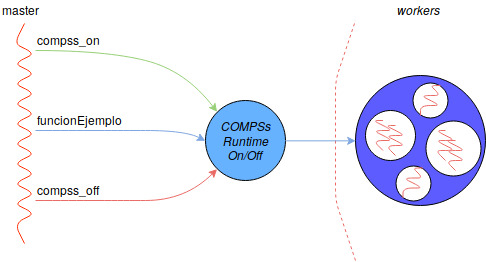
\includegraphics[width=\textwidth]{sta-masterworker.jpg}
    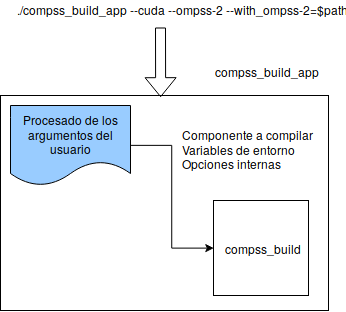
\includegraphics[scale=0.7]{compilation.png}
    \label{fig:compilado}
\end{figure}

En la imagen \ref{fig:compilado} vemos que existen dos \textit{scripts}, \textit{compss\_build\_app} y \textit{compss\_build}, el primero es el encargado de recoger los argumentos que el usuario haya introducido para la compilación de su aplicación (si se utiliza \textit{OmpSs}, donde está la instalación de \textit{OmpSs}, si se utiliza \textit{OpenCL}, o \textit{Cuda}, etc) y procesarlos configurando el entorno correcto para la compilación según estos argumentos que ha introducido el usuario. Una vez configurado el entorno se ejecuta el segundo \textit{script} \textit{compss\_build} tanto para el \textit{master} como para el \textit{worker}, que será realmente quién efectúe la compilación. 
\par\bigskip
Para ello se utiliza un conjunto de herramientas muy populares desarrolladas por \textit{GNU},  \textit{Autotools} \ref{appendix:autotools}. Estas herramientas tienen como objetivo facilitar a los usuarios (que no a los desarrolladores...) la compilación y portabilidad entre plataformas. Pese a que es un campo interesante y muy útil, no entraremos demasiado en detalles, daremos una visión general y entraremos en las modificaciones que se han realizado con tal de poder compilar aplicaciones del tipo \textit{COMPSs+OmpSs-2}. 
\par\bigskip
Como ya hemos visto, \textit{compss\_build\_app} hace de alguna manera de \textit{wrapper} de \textit{compss\_build}, es decir, lo ejecuta con los parámetros adecuados las veces que sea necesario. Este segundo, es el que toca de primera mano \textit{Autotools}, con tal de utilizarlo para compilar una aplicación hay que generar una serie de ficheros. La siguiente imagen nos muestra una porción del \textit{script}  \textit{compss\_build} para generar el \textit{script} \textit{autogen.sh}, que al ser ejecutado nos generará estos ficheros que \textit{Autotools} necesita.
\smallskip

\begin{lstlisting} [caption={Porción del script autogen.sh que genera los ficheros base necesarios para Autotools.},captionpos=b, label={lst:aclocal}, language=bash]
/bin/cat > autogen.sh << EOF
#!/bin/bash
set -e

/usr/bin/aclocal
/usr/bin/automake -a -c
/usr/bin/autoconf
EOF       
\end{lstlisting}

La primera y la última línea de la imagen \ref{lst:aclocal} sirven para escribir el código contenido entre estas en el fichero \textit{autogen.sh}. El \textit{script} \textit{autogen.sh} es generado por \textit{compss\_build} cada vez que se quiere compilar una aplicación y también en función de si se está compilando el \textit{master} o el \textit{worker} (de hecho, se encuentran en sitios distintos), tendrá una forma u otra. 
\par\smallskip

Una vez ejecutada esta porción del \textit{script} \textit{autogen.sh}, entre otros, esto nos habrá generado un \textit{script} \textit{configure}, que al ser ejecutado generará un \textit{Makefile} adaptado al entorno que hayamos especificado. Nuestro proceso de compilado requiere ser flexible, ya que permitimos utilizar \textit{OmpSs}, a veces con \textit{Cuda}, a veces con \textit{OpenCL}... Por tanto, necesitamos pasarle al compilador dónde se encuentran las librerías que necesitamos, \textit{flags} adicionales que necesitemos (\textit{-{}-ompss}, \textit{-{}-ompss-2}, \textit{-{}-cuda}...). Por suerte, este \textit{configure}, nos permite pasar variables de entorno a tener en cuenta durante la compilación, además de opciones personalizadas, a continuación del código de la imagen \ref{lst:aclocal} añadiremos código para que \textit{autogen.sh} ejecute el \textit{script} \textit{configure} con las opciones que necesitamos.
\par\bigskip

\begin{lstlisting} [caption={Porción del script autogen.sh que se encarga de customizar la ejecución de configure.},captionpos=b, label={lst:customconfigure}, language=bash]                                                                                                                                               
if [ "$OMPSS2_ENABLED" == "enabled" ]; then
    ldflags_aux="$ldflags_aux -L$OMPSS2_DIR/lib
                -Wl,-rpath,$OMPSS2_DIR/lib"
    cflags_aux="$cflags_aux -I$OMPSS2_DIR/include"
    conf_opts="--with-ompss-2"
fi

if [ "$OMPSS_ENABLED" == "enabled" ]; then
    ldflags_aux="$ldflags_aux -L$OMPSS_DIR/lib"
    cflags_aux="$cflags_aux -I$OMPSS_DIR/include"
    conf_opts="$conf_opts --with-ompss"
fi

if [ "$CUDA_ENABLED" == "enabled" ]; then
    ldflags_aux="$ldflags_aux -L$CUDA_HOME/lib64"
    cflags_aux="$cflags_aux -I$CUDA_HOME/include"
    conf_opts="$conf_opts --with-cuda"
fi

/bin/cat >> autogen.sh << EOF
./configure --with-cs-prefix=$CS_HOME $conf_opts \ 
            CXXFLAGS="$CXXFLAGS $cflags_aux"     \  
            CFLAGS="$CFLAGS $cflags_aux"         \
            LDFLAGS="$LDFLAGS $ldflags_aux" 
EOF

/bin/chmod +x autogen.sh
\end{lstlisting}

Anteriormente hemos mencionado que el \textit{script} \textit{compss\_build\_app} es el encargado de recolectar los \textit{flags} que nos interesan del usuario en el proceso de compilación y servirlos al \textit{script} \textit{compss\_build}, como se puede ver en la imagen \ref{lst:customconfigure} en función de si las variables de entorno \textit{OMPSS2\_ENABLED}, \textit{OMPSS\_ENABLED}, o \textit{CUDA\_ENABLED} tienen por valor la cadena de carácteres \textit{enabled}, definirá el valor de los \textit{flags} para la fase de compilación \textit{CXXFLAGS} y \textit{CFLAGS}, que se asignarán via la variable \textit{cflags\_aux} y para la fase de \textit{linking} \textit{LDFLAGS} que se asignará via la variable \textit{ldflags\_aux}, además de las opciones personalizadas (que serán pasadas mediante la variable \textit{conf\_opts}).
\par\smallskip
Dos ficheros esenciales en todo este proceso, son \textit{configure.ac} y \textit{Makefile.am}, uno utiliza una serie de \textit{macros} para generar de manera customizada \textit{configure} (por ejemplo, con las opciones mencionadas anteriormente), y el otro indica cuáles son los ficheros que deben ser compilados, cómo y adónde irán una vez compilados.
\par\bigskip
Las modificaciones que explicamos ahora mismo sólo se han aplicado al \textit{worker}, para el \textit{master} no se ha necesitado ningún tipo de modificación. Para declarar una opción personalizada en \textit{configure} se utiliza la macro \textit{AC\_ARG\_WITH}, que tiene como argumentos el nombre de la opción (ompss, que pasará a ser with-ompss), el mensaje de ayuda para el usuario y lo que hay que hacer en caso que se habilite la opción, la imagen \ref{lst:ac-ompss} muestra exactamente cómo se hace.
\bigskip
Para el resto de opciones se utiliza el mismo mecanismo, pero las acciones a realizar si se habilita la opción son distintas. Con tal de compilar una aplicación de \textit{OmpSs-2} necesitamos librerías de \textit{Pthreads}, \textit{dl}\footnote{https://en.wikipedia.org/wiki/Dynamic\_loading}, \textit{nanos6} (evidentemente para todo lo que concierne al \textit{runtime}), y \textit{custom-nanos6}, que no es más que la adaptación a librería del \textit{nanos6-library-mode.o} que se utilizó en la sección \ref{sec:compilado}. La imagen \ref{lst:ac-ompss-2} muestra exactamente cómo lo hacemos.
\bigskip

En este caso a parte de la macro \textit{AC\_ARG\_WITH} se utiliza \textit{AC\_CHECK\_LIB}, esta macro hará que se compruebe si la librería del primer argumento existe y contiene la función del segundo argumento, el tercer y el cuarto argumento indican respectivamente que se hará si se encuentra la librería y que se hará en caso que no se encuentre. Nótese que esta macro, añade la librería a la variable de entorno \textit{LIBS} (librerías que tomarán parte en la fase de \textit{linking}). En el caso de cuda debemos buscar la librería del \textit{runtime} de \textit{Cuda}, que es \textit{cudart}. Se utilizan exactamente los mismos mecanismos que en el resto de opciones, se muestra exactamente en la imagen \ref{lst:ac-cuda}.

\bigskip

Para todas las opciones, en las imágenes \ref{lst:ac-ompss}, \ref{lst:ac-ompss-2} y \ref{lst:ac-cuda} se asigna el valor a una variable ompss, ompss-2 y cuda respectivamente para cada opción al valor \textit{true}. Con la macro \textit{AC\_CONDITIONAL} asignamos a una variable con el nombre del primer argumento el valor que obtengamos del segundo. Estas variables son visibles en el fichero \textit{Makefile.am}, de manera que podremos condicionar la compilación en función de que opciones pase el usuario al \textit{script} \textit{configure}.

\bigskip

Esto sería todo lo relacionado con el \textit{configure.ac}, ahora entraríamos con el \textit{Makefile.am}. Recordemos que lo único que necesitamos compilar con \textit{-{}-ompss-2} es el fichero que contiene las funciones a ser ejecutadas como tareas, por lo tanto necesitamos hacer una distinción de los \textit{flags} que se utilizan para compilar este fichero. Para conseguir esto, hemos decidido indicar en el \textit{Makefile.am} que se haga una librería de este fichero y se compile con unos \textit{flags} en especial, para así aislarlo del resto. En la siguiente imagen se muestra como se hace esto.


\bigskip

La primera librería indica que \textit{libfunctions.a} es una librería que no debe ser instalada, y la segunda que el fichero fuente de esta librería es \textit{PACKAGE-functions.cc} donde \textit{PACKAGE} es el nombre del paquete. Las siguientes líneas indican los \textit{flags} base que se utilizarán para compilar los ficheros fuente. 
\smallskip

A esta altura, ya tenemos la base para compilar la librería, pero si no podemos poner los \textit{flags} para \textit{OmpSs-2} o \textit{OmpSs} no habremos conseguido nada. Utilizaremos las variables que hemos definido anteriormente en \ref{lst:ac-vars}. Sencillamente, en función de si las variables correspondientes tienen el valor adecuado, añadimos a las variables adecuadas los \textit{flags} que requerimos. Por ejemplo, si el usuario está compilando con \textit{OmpSs-2}, los \textit{flags} para compilar \textit{libfunctions.a} deben contener \textit{-{}-ompss-2} entre otros. En la imagen \ref{lst:am-cond-flags} se procede a asignar los \textit{flags} de esta manera.

\bigskip

Está claro que después de haber compilado la libería habrá que hacer el \textit{linking} de ella con \textit{nio\_worker\_c} o \textit{worker\_c}. Con esto ya habríamos hecho las modificaciones necesarias para poder compilar la aplicación de \textit{COMPSs+OmpSs-2}.

\subsubsection{Tipo enum y cabeceras en la interfaz}

\todo{pongo detalles? O solo explico por encima}

Un añadido al proyecto ha sido soportar el tipo \textit{enum} y añadir la posibilidad de incluir cabeceras en la interfaz de una aplicación \textit{C/C++}. Para hacer esto, ha habido que hacer modificaciones en la gramática del compilador y en la generación de código. Este añadido puede ser muy útil para cuando se utilicen librerías externas en la interfaz y se precise de cabeceras adicionales que incluyan tipos que se necesitan.
\bigskip
El compilador está hecho con las herramientas \textit{Lex} un generador de analizadores léxicos y \textit{Yacc} un generador de analizadores sintácticos, es decir, las dos piezas fundamentales para hacer un compilador, ya que uno nos facilitará crear un autómata para la gramática de la interfaz y el otro nos permite comprobar que realmente tiene sentido la interfaz escrita.
\bigskip
Para añadir el tipo \textit{enum}, hemos tenido que permitir que la gramática reconozca algo del estilo "\textit{in/out enum} tipo nombre\_variable", una vez hecho esto ya solo hay que asociar el comportamiento que el compilador tiene con el tipo entero al del \textit{enum}, ya que al final ambos son enteros. De forma similar, para el \textit{include} hubo que hacer que la gramática reconociera un patrón "\textit{include} nombre\_cabecera;" y al generar el código incluir la cabecera.


\subsection{Estudio previo del rendimiento}

En la sección \ref{sec:compssompss} se enunciaron los problemas que tuvimos con la integración inicial \textit{COMPSs+OmpSs}. En este apartado, se realiza un estudio previo del rendimiento para saber si finalmente estos problemas están resueltos con la nueva integración. Para ello, hemos desarrollado una aplicación con dos tareas de diferente granularidad, con \textit{Extrae} y \textit{Paraver} veremos como se comporta la integración ante este caso. A grandes rasgos, la aplicación básicamente ejecuta 30 tareas de granularidad fina y gruesa, ésta se emula haciendo un \textit{usleep} de 50000 y 300000 microsegundos respectivamente. La implementación se encuentra en el apéndice \ref{appendix:estudioprevio}.
\par\bigskip
Entonces, en una ejecución de esta aplicación, si sacásemos una traza, el tiempo que dura cada traza debería ser notoriamente distinto, del orden de la espera que hacen cada una. La siguiente imagen muestra una traza de \textit{COMPSs} en la cuál se han utilizado 12 CPUs para la ejecución.

\begin{figure}[H]
	\centering 
	\caption{Traza COMPSs con 12 CPUs.}
	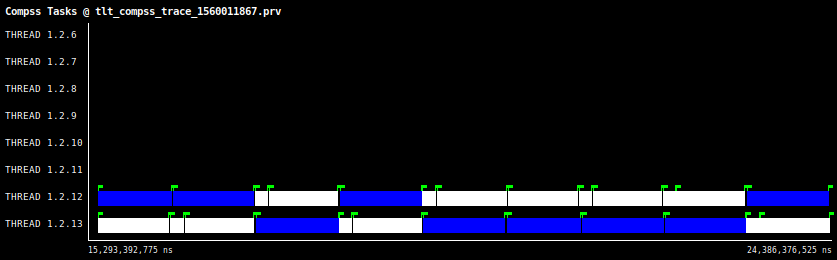
\includegraphics[scale=0.4]{estudio_previo/NER_COMPSS_TLT.png}
	\label{fig:tltcompss12cpus}
\end{figure}

En esta traza, los bloques azules son las tareas de granularidad gruesa y de color blanco, fina. El tamaño hace referencia a la duración de la tarea, si nos fijamos, las de granularidad fina tienen una duración muy irregular y a veces es similar a las de granularidad gruesa, esto no tiene sentido. Con tal de investigar por qué sucede esto, vamos a sacar una traza de la misma ejecución pero de \textit{OmpSs-2}.

\begin{figure}[H]
	\centering 
	\caption{Traza OmpSs-2 con 12 CPUs.}
	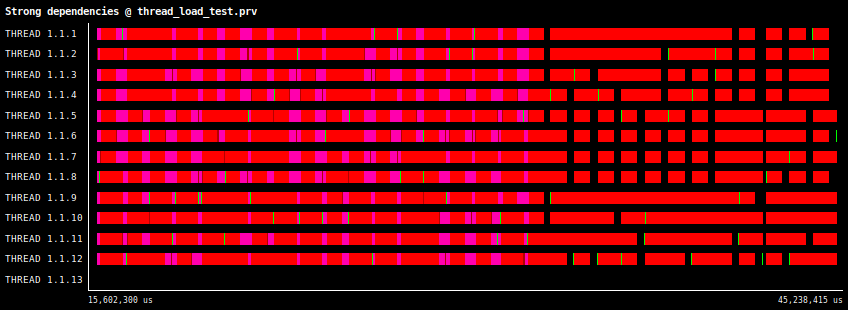
\includegraphics[scale=0.4]{estudio_previo/NER_OmpSs-2_TLT.png}
	\label{fig:tltompss12cpus}
\end{figure}

Los bloques de color rojo son las tareas de granularidad gruesa y los de color rosa, fina. Si nos fijamos bien hay incluso de color verde claro y un rojo más oscuro, pero estas tareas hacen referencia al \textit{spawn} por lo que no tienen importancia en este caso. Recordemos que dentro de un mismo nodo, se comparte el \textit{runtime} de \textit{OmpSs-2} por lo cuál las tareas de \textit{COMPSs} que se ejecutan en un mismo nodo están sujetas a \textit{OmpSs-2}. El hecho de que las tareas de \textit{COMPSs} tarden más o menos, es así por que \textit{OmpSs-2} constantemente ejecuta tareas en las CPUs que le parece mejor para explotar el paralelismo dentro del nodo, haciendo que una tarea de \textit{COMPSs} que podría ejecutar tan sólo lo que a ella le concierne ejecute también trabajo del resto, prolongando su duración (lo que vimos en la traza \ref{fig:tltcompss12cpus}).
\par\bigskip
Esto que hemos visto, ha sucedido cuando teníamos 12 CPUs, pero ¿Qué pasaría si en vez de 12 tuviéramos 160? Puesto que la situación anterior es provocada por cómo \textit{OmpSs-2} gestiona los recursos, seguramente si tuviéramos más, observaríamos un comportamiento más parecido al que habíamos pensado en primer momento.
\par\bigskip

\begin{figure}[H]
	\centering 
	\caption{Traza COMPSs con 160 CPUs.}
	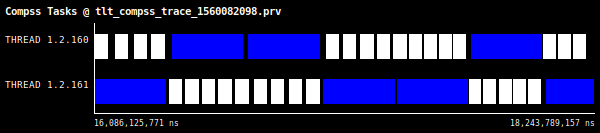
\includegraphics[scale=0.6]{estudio_previo/ER_COMPSS_TLT.png}
	\label{fig:tltcompss160cpus}
\end{figure}

Si la comparamos con la traza \ref{fig:tltcompss12cpus}, la duración de las tareas es mucho más regular, siempre son de la misma magnitud, y nunca una tarea de granularidad fina dura más que una gruesa. Esto se debe a que tenemos más recursos, y por lo general no hay dos o más tareas que necesiten una misma CPU al mismo momento, por lo cuál no se nos alargan las tareas de \textit{COMPSs}. En la siguiente imagen se muestra una traza desde el punto de vista de \textit{OmpSs-2}.

\begin{figure}[H]
	\centering 
	\caption{Traza OmpSs-2 con 160 CPUs.}
	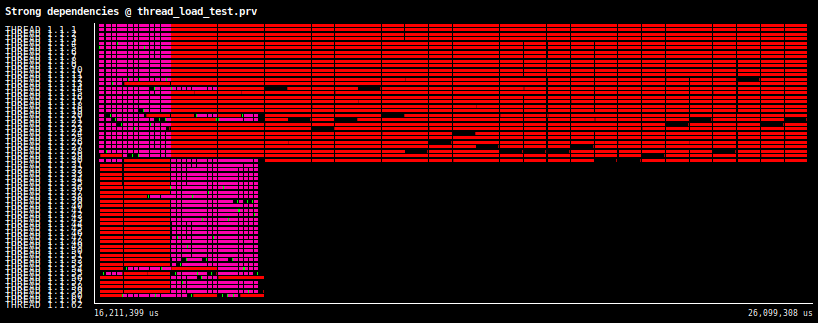
\includegraphics[scale=0.45]{estudio_previo/ER_OmpSs-2_TLT.png}
	\label{fig:tltompss160cpus}
\end{figure}

Hay una diferenciación mucho más clara entre los dos tipos de tareas, y por lo general no existen estos conflictos por recursos que comentábamos. De todas formas, el comportamiento negativo que se ha enunciado con el primer par de trazas puede suceder eventualmente, ya que la manera en la que se gestionan los recursos no ha cambiado, pero mejora mucho.
\par\bigskip
No hemos solucionado uno de los problemas que enunciamos, pero esto no quiere decir que la nueva integración no aporte mejoras en el rendimiento. Para decidir si realmente lo que hemos visto en estas trazas es un comportamiento negativo para \textit{COMPSs}, deberemos efectuar el estudio de rendimiento en comparación con \textit{COMPSs+OmpSs}.

\section{Aplicación COMPSs+OmpSs-2}

Para verificar el funcionamiento de las funcionalidades y el rendimiento de la integración \textit{COMPSs+OmpSs-2}, hemos desarrollado dos aplicaciones, \textit{K-Means} y \textit{Cholesky}.

\subsection{K-Means}



\subsection{Cholesky}



\section{Estudio del rendimiento}

